\documentclass[aspectratio=169,11pt]{beamer}

% --- Minimal look -----------------------------------------------------------
\usetheme{default}
\usefonttheme{professionalfonts}
\setbeamertemplate{navigation symbols}{}
\setbeamertemplate{footline}[frame number]
\setbeamertemplate{itemize items}[circle]
\setbeamertemplate{bibliography item}{}
\setbeamercolor{frametitle}{fg=black}
\setbeamercolor{title}{fg=black}
\setbeamercolor{structure}{fg=black!70}
\setbeamercolor{alerted text}{fg=red!60!black}
\setbeamerfont{frametitle}{series=\bfseries}
\setbeamercolor{block title}{fg=black,bg=black!8}
\setbeamercolor{block body}{bg=black!3}

% --- Packages ---------------------------------------------------------------
\usepackage[utf8]{inputenc}
\usepackage[T1]{fontenc}
\usepackage{lmodern}
\usepackage{amsmath,amssymb}
\usepackage{booktabs}
\usepackage{graphicx}
\usepackage{tikz}
\usetikzlibrary{calc,arrows.meta,positioning}
\usepackage[authoryear,round]{natbib}

% --- Math shortcuts ---------------------------------------------------------
\newcommand{\R}{\mathbb{R}}
\newcommand{\Orth}{\mathrm{O}}

% --- Architecture diagrams (same color coding as Fig. 1 of the SAN paper) ----
\definecolor{lpe}{RGB}{169,209,142}
\definecolor{mainT}{RGB}{244,177,131}
\tikzset{
  flow/.style={-{Stealth[length=1.6mm]},thick,black!60},
  op/.style={draw,rounded corners=2pt,align=center,font=\scriptsize,inner sep=3pt,minimum height=8mm},
  dim/.style={font=\scriptsize},
  cell/.style={draw,minimum height=4mm,inner sep=0pt,font=\scriptsize}
}
% One matrix "sheet": \sheet{x}{y}{width}{fill}; rows are the m eigenpairs.
\newcommand{\sheet}[4]{
  \foreach \s in {2,1} \draw[fill=white] ($(#1,#2)+(\s*0.07,\s*0.07)$) rectangle ++(#3,-1.5);
  \draw[fill=#4] (#1,#2) rectangle ++(#3,-1.5);
  \foreach \r in {0.3,0.6,0.9,1.2} \draw[black!40] (#1,#2-\r) -- ++(#3,0);
}

% --- Title ------------------------------------------------------------------
\title{Survey on Spectral Geometry as Positional Encoding\\in Graph Transformers}
\author{Gabriele Moisè}
\institute{Università degli Studi di Milano-Bicocca}
\date{}

\begin{document}

\begin{frame}[plain]
  \titlepage
\end{frame}

\begin{frame}{Outline}
  \tableofcontents
\end{frame}

% ============================================================================
\section{Motivation}

\begin{frame}{Expressive power of message passing}
  \begin{itemize}
    \item Message-passing GNNs are at most as expressive as the
          \alert{1-Weisfeiler--Leman (1-WL)} graph isomorphism test
          \citep{xu2019powerful}.
    \item 1-WL iteratively refines node colors and compares the resulting
          histograms:
          \begin{itemize}
            \item different histograms $\Rightarrow$ graphs are \emph{not} isomorphic;
            \item same histogram $\Rightarrow$ graphs \emph{may} be isomorphic.
          \end{itemize}
    \item If 1-WL maps two graphs to the same histogram, an MPNN cannot
          distinguish them.
  \end{itemize}
\end{frame}

\begin{frame}{A failure case of 1-WL}
  \centering
  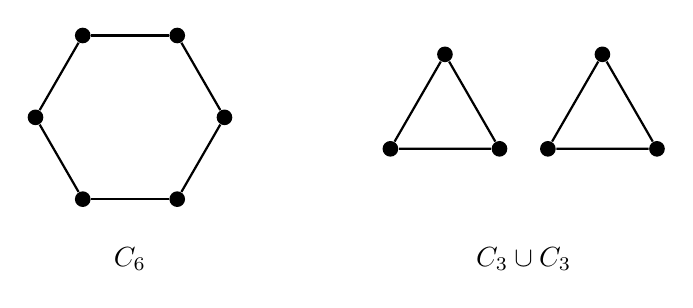
\begin{tikzpicture}[
      v/.style={circle,fill=black,inner sep=2pt},
      e/.style={thick}]
    % Hexagon
    \foreach \i in {0,...,5}
      \node[v] (h\i) at ({60*\i}:1.2) {};
    \foreach \i [evaluate=\i as \j using {int(mod(\i+1,6))}] in {0,...,5}
      \draw[e] (h\i) -- (h\j);
    \node at (0,-1.8) {$C_6$};

    % Two triangles
    \begin{scope}[xshift=5cm]
      \foreach \i in {0,1,2}
        \node[v] (a\i) at ($(-1,0)+({90+120*\i}:0.8)$) {};
      \foreach \i in {0,1,2}
        \node[v] (b\i) at ($(1,0)+({90+120*\i}:0.8)$) {};
      \draw[e] (a0)--(a1)--(a2)--(a0);
      \draw[e] (b0)--(b1)--(b2)--(b0);
      \node at (0,-1.8) {$C_3 \cup C_3$};
    \end{scope}
  \end{tikzpicture}

  \bigskip
  Every node has degree 2 in both graphs, so 1-WL (and any MPNN) cannot tell
  them apart.\\
  \alert{Positional encodings} inject the structural information that message
  passing misses.
\end{frame}

% ============================================================================
\section{Spectral Attention Network}

\begin{frame}{The starting point: Attention Is All You Need}
  \centering
  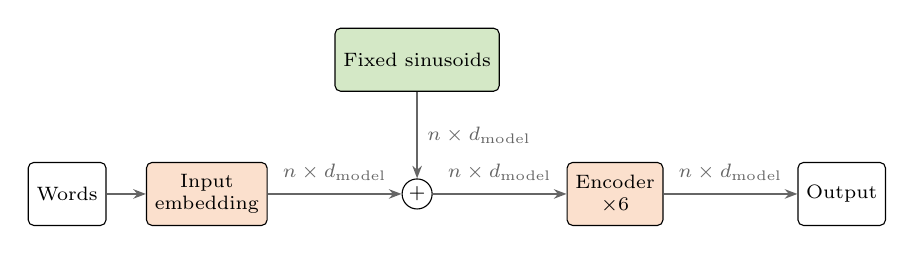
\begin{tikzpicture}[node distance=5mm]
    \node[op] (tok) {Words};
    \node[op,right=of tok,fill=mainT!40] (emb) {Input\\embedding};
    \node[op,right=17mm of emb,circle,minimum height=0pt,inner sep=1pt] (plus) {$+$};
    \node[op,above=11mm of plus,fill=lpe!50] (pe) {Fixed sinusoids};
    \node[op,right=17mm of plus,fill=mainT!40] (enc) {Encoder\\$\times 6$};
    \node[op,right=17mm of enc] (out) {Output};
    \draw[flow] (tok) -- (emb);
    \draw[flow] (emb) -- node[dim,above=1pt] {$n \times d_{\text{model}}$} (plus);
    \draw[flow] (pe) -- node[dim,right] {$n \times d_{\text{model}}$} (plus);
    \draw[flow] (plus) -- node[dim,above=1pt] {$n \times d_{\text{model}}$} (enc);
    \draw[flow] (enc) -- node[dim,above=1pt] {$n \times d_{\text{model}}$} (out);
  \end{tikzpicture}

  \medskip
  {\small $PE_{(pos,2i)} = \sin\!\big(pos / 10000^{2i/d_{\text{model}}}\big), \quad
  PE_{(pos,2i+1)} = \cos\!\big(pos / 10000^{2i/d_{\text{model}}}\big)$
  \quad ($d_{\text{model}} = 512$)}

  \raggedright
  \medskip
  \begin{itemize}
    \item A sequence has a natural order, so $pos$ is an integer and the
          frequencies can be \alert{fixed in advance}
          \citep{vaswani2017attention}.
    \item PE and embedding have the \alert{same size}, so they can be summed.
    \item A graph has no $pos$, and each graph has \alert{its own frequencies}.
          What replaces the sinusoids?
  \end{itemize}
\end{frame}

\begin{frame}{From sinusoids to Laplacian eigenfunctions}
  \begin{itemize}
    \item In Euclidean space, the eigenfunctions of the Laplacian \emph{are}
          sinusoids, with eigenvalues given by the squared frequencies.
    \item On a graph, the natural equivalent is the eigenvectors $\phi_i$ of
          $L$ \citep{kreuzer2021rethinking}.
  \end{itemize}

  \medskip
  \centering
  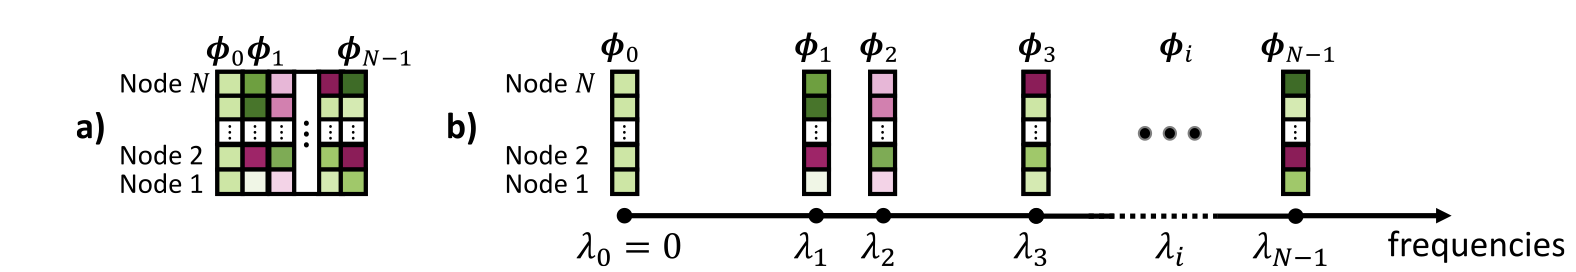
\includegraphics[width=0.92\textwidth]{figures/san_fig2.png}

  {\scriptsize \citet[Fig.~2]{kreuzer2021rethinking}: (a) eigenvectors as a matrix,
  (b) eigenvectors placed on the axis of eigenvalues.}

  \medskip
  \raggedright
  \textbf{Key idea:} (b) is a \alert{sequence}, with non-uniform positions given by
  $\lambda_i$. Sequences are what Transformers process.
\end{frame}

\begin{frame}{SAN: two Transformers}
  \begin{columns}[c]
    \begin{column}{0.68\textwidth}
      \centering
      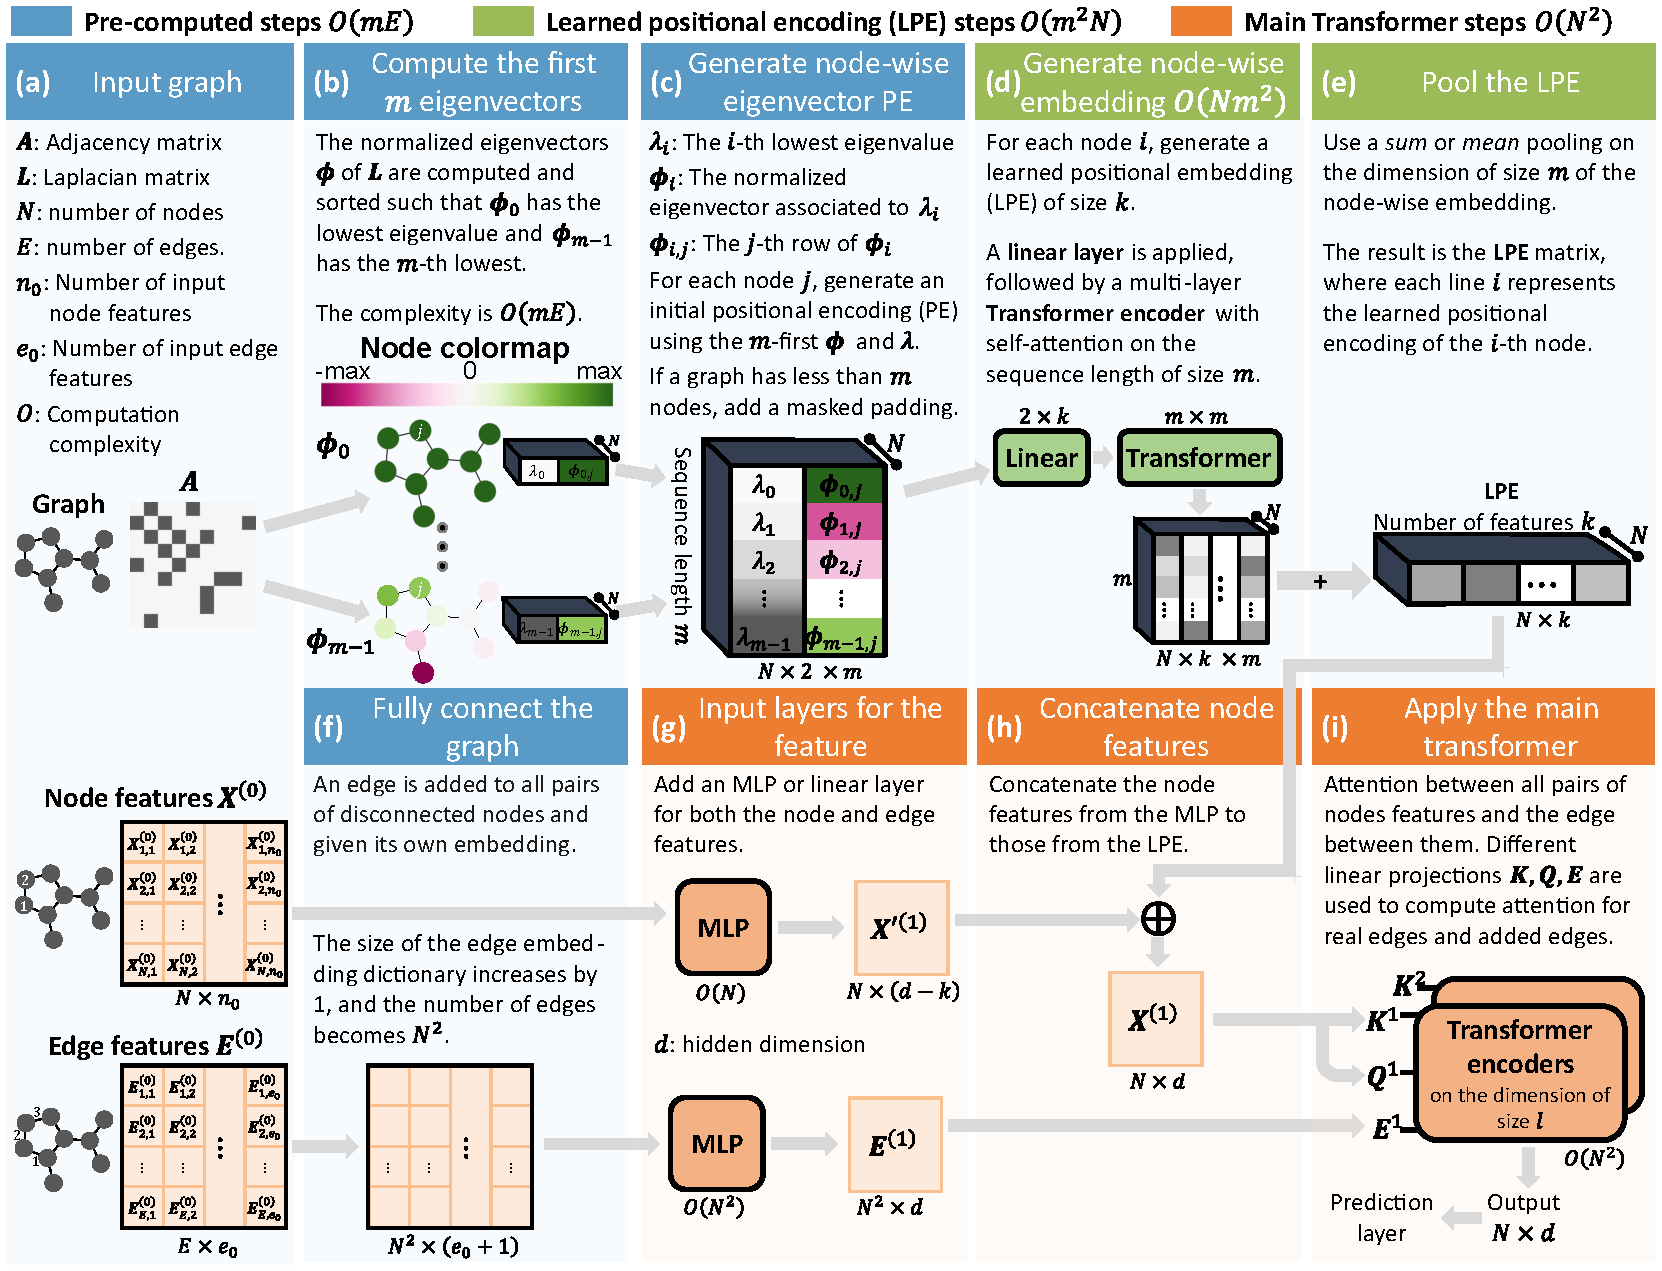
\includegraphics[height=0.84\textheight]{figures/san_fig1.png}
    \end{column}
    \begin{column}{0.3\textwidth}
      \small
      \tikz\fill[lpe] (0,0) rectangle (0.3,0.2); \textbf{LPE Transformer}\\
      attention over the $m$ eigenpairs of each node

      \medskip
      \tikz\fill[mainT] (0,0) rectangle (0.3,0.2); \textbf{Main Transformer}\\
      attention over all pairs of the $N$ nodes

      \bigskip
      \scriptsize Figure: \citet[Fig.~1]{kreuzer2021rethinking}.
    \end{column}
  \end{columns}
\end{frame}

\begin{frame}{Learned Positional Encoding: following the dimensions}
  \centering
  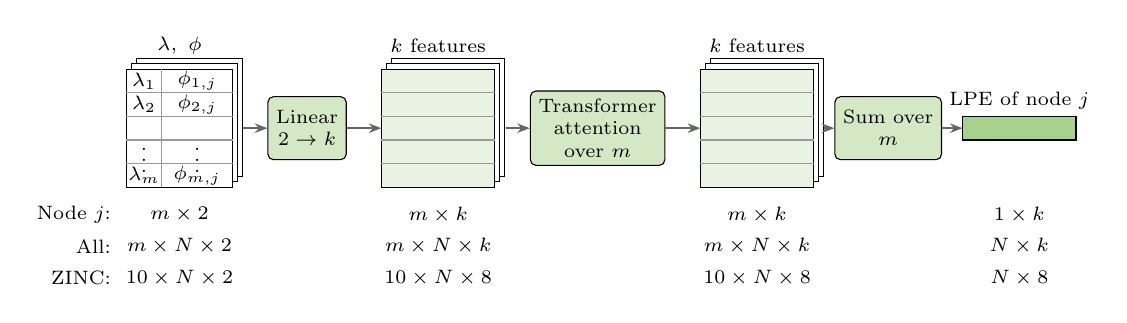
\begin{tikzpicture}[x=0.9cm,y=1cm]
    % Input
    \sheet{0}{0}{1.5}{white}
    \draw[black!40] (0.5,0) -- ++(0,-1.5);
    \node[dim] at (0.25,-0.15) {$\lambda_1$};
    \node[dim] at (1.0,-0.15) {$\phi_{1,j}$};
    \node[dim] at (0.25,-0.45) {$\lambda_2$};
    \node[dim] at (1.0,-0.45) {$\phi_{2,j}$};
    \node[dim] at (0.25,-1.05) {$\vdots$};
    \node[dim] at (1.0,-1.05) {$\vdots$};
    \node[dim] at (0.25,-1.35) {$\lambda_m$};
    \node[dim] at (1.0,-1.35) {$\phi_{m,j}$};
    % Linear
    \node[op,fill=lpe!50] (lin) at (2.55,-0.75) {Linear\\$2 \to k$};
    % After linear
    \sheet{3.6}{0}{1.6}{lpe!25}
    % Transformer
    \node[op,fill=lpe!50] (tr) at (6.65,-0.75) {Transformer\\attention\\over $m$};
    % After transformer
    \sheet{8.1}{0}{1.6}{lpe!25}
    % Pool
    \node[op,fill=lpe!50] (pool) at (10.75,-0.75) {Sum over\\$m$};
    % LPE
    \draw[fill=lpe] (11.8,-0.6) rectangle ++(1.6,-0.3);
    \node[dim] at (12.6,-0.4) {LPE of node $j$};
    % Sheet sizes
    \node[dim] at (4.4,0.3) {$k$ features};
    \node[dim] at (8.9,0.3) {$k$ features};
    \node[dim] at (0.75,0.3) {$\lambda,\ \phi$};
    % Arrows
    \draw[flow] (1.65,-0.75) -- (lin);
    \draw[flow] (lin) -- (3.6,-0.75);
    \draw[flow] (5.35,-0.75) -- (tr);
    \draw[flow] (tr) -- (8.1,-0.75);
    \draw[flow] (9.85,-0.75) -- (pool);
    \draw[flow] (pool) -- (11.8,-0.75);
    % Dimensions
    \node[dim,anchor=east] at (-0.08,-1.85) {Node $j$:};
    \node[dim] at (0.75,-1.85) {$m \times 2$};
    \node[dim] at (4.4,-1.85) {$m \times k$};
    \node[dim] at (8.9,-1.85) {$m \times k$};
    \node[dim] at (12.6,-1.85) {$1 \times k$};
    \node[dim,anchor=east] at (-0.08,-2.25) {All:};
    \node[dim] at (0.75,-2.25) {$m \times N \times 2$};
    \node[dim] at (4.4,-2.25) {$m \times N \times k$};
    \node[dim] at (8.9,-2.25) {$m \times N \times k$};
    \node[dim] at (12.6,-2.25) {$N \times k$};
    \node[dim,anchor=east] at (-0.08,-2.65) {ZINC:};
    \node[dim] at (0.75,-2.65) {$10 \times N \times 2$};
    \node[dim] at (4.4,-2.65) {$10 \times N \times 8$};
    \node[dim] at (8.9,-2.65) {$10 \times N \times 8$};
    \node[dim] at (12.6,-2.65) {$N \times 8$};
  \end{tikzpicture}

  \raggedright
  \medskip
  \begin{itemize}
    \item $m$ is the \alert{sequence length} (eigenpairs); $N$ acts as the
          \alert{batch} (the same network runs on every node); $k$ is the hidden size.
    \item No separate PE: $\lambda_i$ is an input channel, so \alert{it is the position}.
    \item If $N < m$, the missing eigenpairs are masked. Cost: $O(m^2 N)$.
  \end{itemize}
\end{frame}

\begin{frame}[fragile]{How the LPE enters the embedding}
  \centering
  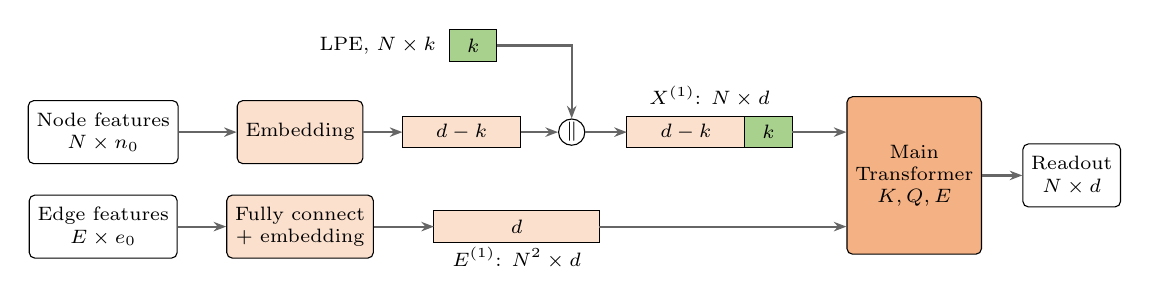
\begin{tikzpicture}[x=1cm,y=1cm]
    % Node row
    \node[op] (x0) at (0.7,0) {Node features\\$N \times n_0$};
    \node[op,fill=mainT!40] (mlpx) at (3.2,0) {Embedding};
    \draw[fill=mainT!40] (4.5,0.2) rectangle node[dim] {$d-k$} ++(1.5,-0.4);
    \draw[fill=lpe] (5.1,1.3) rectangle node[dim] {$k$} ++(0.6,-0.4);
    \node[dim,anchor=east] at (5.05,1.1) {LPE, $N \times k$};
    \node[op,circle,minimum height=0pt,inner sep=0.5pt] (cat) at (6.65,0) {$\Vert$};
    \draw[fill=mainT!40] (7.35,0.2) rectangle node[dim] {$d-k$} ++(1.5,-0.4);
    \draw[fill=lpe] (8.85,0.2) rectangle node[dim] {$k$} ++(0.6,-0.4);
    \node[dim] at (8.4,0.45) {$X^{(1)}$: $N \times d$};
    \node[op,fill=mainT,minimum height=20mm] (main) at (11,-0.55) {Main\\Transformer\\$K, Q, E$};
    \node[op] (out) at (13,-0.55) {Readout\\$N \times d$};
    % Edge row
    \node[op] (e0) at (0.7,-1.2) {Edge features\\$E \times e_0$};
    \node[op,fill=mainT!40] (mlpe) at (3.2,-1.2) {Fully connect\\+ embedding};
    \draw[fill=mainT!40] (4.9,-1) rectangle node[dim] {$d$} ++(2.1,-0.4);
    \node[dim] at (5.95,-1.6) {$E^{(1)}$: $N^2 \times d$};
    % Arrows
    \draw[flow] (x0) -- (mlpx);
    \draw[flow] (mlpx) -- (4.5,0);
    \draw[flow] (6,0) -- (cat);
    \draw[flow] (5.7,1.1) -| (cat);
    \draw[flow] (cat) -- (7.35,0);
    \draw[flow] (9.45,0) -- (main.west |- 0,0);
    \draw[flow] (e0) -- (mlpe);
    \draw[flow] (mlpe) -- (4.9,-1.2);
    \draw[flow] (7,-1.2) -- (main.west |- 0,-1.2);
    \draw[flow] (main) -- (out);
  \end{tikzpicture}

  \raggedright
  \medskip
  \begin{itemize}
    \item The node embedding is \alert{shortened by $k$} to make room for the
          LPE (ZINC: $48 + 8 = 56$).
    \item Unlike \citet{vaswani2017attention}, the PE is \alert{concatenated}, not
          summed: it gets its own $k$ dimensions.
  \end{itemize}

  \vspace{-1mm}
\begin{verbatim}
self.embedding_h = nn.Embedding(num_atom_type, GT_hidden_dim-LPE_dim)
h = torch.cat((h, PosEnc), 1)   # N x (d-k) + N x k = N x d
\end{verbatim}
\end{frame}

\begin{frame}{Same blueprint as Attention Is All You Need}
  \centering
  \footnotesize
  \begin{tabular}{llll}
    \toprule
    & \textbf{Attention Is All You Need} & \textbf{SAN: LPE} & \textbf{SAN: main} \\
    \midrule
    Sequence elements & $n$ words & $m$ eigenpairs & $N$ nodes \\
    Batch dimension   & sentences & nodes & graphs \\
    Hidden size       & $d_{\text{model}} = 512$ & $k$ (ZINC: 8) & $d$ (ZINC: 56) \\
    Position          & integer $pos$ & eigenvalue $\lambda_i$ & LPE vector \\
    Position source   & fixed sinusoids & given by the spectrum & learned \\
    Combination       & sum & concatenation & concatenation \\
    Attention over    & all words & all eigenpairs of a node & all node pairs \\
    Decoder           & yes & no & no \\
    \bottomrule
  \end{tabular}

  \bigskip
  \normalsize
  \raggedright
  \begin{itemize}
    \item The LPE is a standard Transformer encoder, applied along the
          \alert{frequency axis} rather than along a sentence.
    \item Its output plays the role of the sinusoids for the main Transformer:
          a \alert{learned} replacement for a fixed formula.
  \end{itemize}
\end{frame}

\begin{frame}{Attention: from sequences to graphs}
  \textbf{Attention Is All You Need}
  \begin{equation*}
    \mathrm{Attention}(Q,K,V) = \mathrm{softmax}\!\left(\frac{QK^\top}{\sqrt{d_k}}\right) V
  \end{equation*}

  \textbf{SAN}: the same scaled dot product, with edge features and two sets of
  projections
  \begin{equation*}
    \hat{w}_{ij} = \frac{Q h_i \circ K h_j \circ E e_{ij}}{\sqrt{d_k}},
    \qquad
    w_{ij} =
    \begin{cases}
      \dfrac{1}{1+\gamma}\,\mathrm{softmax}\big(\sum_{d_k} \hat{w}_{ij}\big) & \text{real edge}\\[2ex]
      \dfrac{\gamma}{1+\gamma}\,\mathrm{softmax}\big(\sum_{d_k} \hat{w}_{ij}\big) & \text{added edge}
    \end{cases}
  \end{equation*}

  \begin{itemize}
    \item Real and added edges have \alert{separate} $Q, K, E$.
    \item $\gamma$ tunes the bias: $\gamma = 0$ is sparse attention, while large
          $\gamma$ favors full attention.
    \item The graph structure enters twice: through the LPE and through the real
          edges.
  \end{itemize}
\end{frame}

\begin{frame}{Excursus: PE on nodes vs.\ on edges}
  \centering
  \footnotesize
  \begin{tabular}{lll}
    \toprule
    & \textbf{Node LPE} & \textbf{Edge LPE} \\
    \midrule
    Type of position & Absolute & Relative \\
    Input per eigenpair & $\lambda_i,\ \phi_{i,j}$ &
      $\lambda_i,\ |\phi_{i,j_1} - \phi_{i,j_2}|,\ \phi_{i,j_1}\phi_{i,j_2}$ \\
    Tensor (batch $=$ nodes or edges) & $m \times N \times 2$ & $m \times N^2 \times 3$ \\
    Linear layer & $2 \to k$ & $3 \to k$ \\
    Output & $N \times k$ & $N^2 \times k$ \\
    Concatenated to & node embedding ($d-k$) & edge embedding ($d-k$) \\
    Sign-invariant & \alert{No} & \alert{Yes} \\
    Cost (fully connected graph) & $O(m^2 N)$ & \alert{$O(m^2 N^2)$} \\
    \bottomrule
  \end{tabular}

  \medskip
  \normalsize
  \raggedright
  \begin{itemize}
    \item Why invariant: $|(-a)-(-b)| = |a-b|$ and $(-a)(-b) = ab$. Only the
          \alert{relative} sign between two nodes survives.
    \item Intuition from the paper: like potential energy, position is meaningful
          only as a \alert{difference}.
    \item The edge LPE is cleaner but expensive: all the repository's optimized
          configurations use the \alert{node LPE}, which needs a sign fix.
  \end{itemize}
\end{frame}

\begin{frame}{Paper vs.\ code: the sign flip}
  \small
  Paper, §3.1: \emph{``we randomly flip the sign of the pre-computed eigenvectors
  during training''}.

  \medskip
  \scriptsize
  \colorbox{black!4}{\parbox{0.97\textwidth}{\ttfamily
    \#random sign flipping\\
    sign\_flip = torch.rand(batch\_EigVecs.size(1)).to(device)\\
    sign\_flip[sign\_flip>=0.5] = 1.0; sign\_flip[sign\_flip<0.5] = -1.0\\
    \textcolor{red!60!black}{\textbf{batch\_EigVecs = batch\_EigVecs * sign\_flip.unsqueeze(0)}\ \ \# missing in ZINC and SBMs}\\
    batch\_scores = model.forward(batch\_graphs, batch\_x, batch\_e, batch\_EigVecs, batch\_EigVals)
  }}

  \medskip
  \centering
  \footnotesize
  \begin{tabular}{lccccc}
    \toprule
    & ZINC & PATTERN & CLUSTER & MOLHIV & MOLPCBA \\
    \midrule
    Optimized config uses & node LPE & node LPE & node LPE & node LPE & node LPE \\
    Flip computed & \checkmark & \checkmark & \checkmark & \checkmark & \checkmark \\
    Flip \alert{applied} & \alert{--} & \alert{--} & \alert{--} & \checkmark & \checkmark \\
    \bottomrule
  \end{tabular}

  \medskip
  \raggedright
  \small
  In the public code, \alert{3 of 5 benchmarks} train the node LPE with no sign
  augmentation, in every commit, despite what the paper states.

  \vfill
  \scriptsize github.com/DevinKreuzer/SAN, commit 6e38329:
  \texttt{train\_ZINC\_graph\_regression.py}, \texttt{train\_SBMs\_node\_classification.py}
  vs.\ \texttt{train\_molhiv.py}, \texttt{train\_molpcba.py}. The public code may not
  be exactly what produced the published results.
\end{frame}

% ============================================================================
\section{Spectral Positional Encodings}

\begin{frame}{Laplacian eigenvectors as positions}
  Normalized graph Laplacian:
  \begin{equation*}
    L = I - D^{-1/2} A D^{-1/2} = V \Lambda V^\top
  \end{equation*}
  \begin{itemize}
    \item Use the first $k$ eigenvectors $V_{:,1:k} \in \R^{n \times k}$ as node
          positions \citep{dwivedi2020generalization}.
    \item Generalizes sinusoidal encodings: eigenvectors of the path graph
          are Fourier modes.
    \item But eigenvectors are \alert{not unique}, and this is the source of
          most obstacles.
  \end{itemize}
\end{frame}

% ============================================================================
\section{Obstacles}

\begin{frame}{Obstacle 1: Sign ambiguity}
  \begin{itemize}
    \item If $v$ is an eigenvector, so is $-v$; the solver returns either one
          depending on implementation details.
    \item A model that is not sign-invariant sees the \alert{same graph as
          different inputs}: parameters oscillate trying to align fluctuating
          features, which hinders convergence.
    \item \textbf{Random sign flipping} as augmentation
          \citep{dwivedi2020generalization,kreuzer2021rethinking}:
          \begin{itemize}
            \item does not solve the problem mathematically; the ambiguity is not granted to be solved
            \item with $k$ eigenvectors there are $2^k$ sign combinations,
                  which slows training exponentially;
            \item spends model capacity on learning an invariance.
          \end{itemize}
  \end{itemize}
\end{frame}

\begin{frame}{Obstacle 2: Basis ambiguity}
  \begin{itemize}
    \item Symmetric graphs often have eigenvalues with multiplicity $d > 1$.
    \item With distinct eigenvalues, each unit eigenvector is unique up to sign.
    \item With multiplicity $d$, \alert{any} rotation or reflection of an
          orthonormal basis is still a valid basis: infinitely many choices.
    \item Consequence: \alert{overfitting}. The network may learn the bases seen
          in training, but fails on a similar graph whose solver returns a
          basis it never saw.
  \end{itemize}

  \begin{block}{Requirement}
    Changing the basis of the input eigenvectors must not change the output.
  \end{block}
\end{frame}

\begin{frame}{Basis ambiguity, geometrically}
  \begin{itemize}
    \item Let $\lambda_i$ have multiplicity $d_i$ with eigenvectors
          $V_i \in \R^{n \times d_i}$. For any $O_i \in \Orth(d_i)$,
          $V_i O_i$ is still an orthonormal basis of the eigenspace.
    \item Collecting all eigenspaces gives the symmetry group
          \begin{equation*}
            \Orth(\lambda) = \bigoplus_i \Orth(d_i)
            = \Big\{ \bigoplus_i O_i : O_i \in \Orth(d_i) \Big\}.
          \end{equation*}
    \item Both $(V, \lambda)$ and $(VQ, \lambda)$, $Q \in \Orth(\lambda)$, are
          valid eigendecompositions.
  \end{itemize}

  \begin{block}{Basis invariance}
    \vspace{-1.2em}
    \begin{equation*}
      f(V, \lambda) = f(VQ, \lambda) \qquad \forall\, Q \in \Orth(\lambda)
    \end{equation*}
  \end{block}
\end{frame}

\begin{frame}{Obstacle 3: Limits of invariant architectures}
  \begin{itemize}
    \item \textbf{SignNet / BasisNet} \citep{lim2023sign} build the invariance
          into the architecture, e.g.\ SignNet uses
          \begin{equation*}
            \phi(v) + \phi(-v).
          \end{equation*}
    \item This is a \alert{strong inductive bias}:
          \begin{itemize}
            \item restricts the class of learnable functions, which limits expressivity;
            \item increases training time, possibly to reach a suboptimal solution.
          \end{itemize}
    \item They have the right symmetries, but ignore that two \alert{similar
          but distinct} Laplacians can produce completely different eigenspaces.
  \end{itemize}
\end{frame}

\begin{frame}{Obstacle 4: Instability to perturbations}
  \begin{itemize}
    \item \textbf{Stability}: a small change of the Laplacian should give a
          small change of the positional encodings. This generalizes basis
          invariance.
    \item If eigenvalues are close (small \alert{spectral gap}), small
          perturbations can produce completely different eigenvectors
          \citep[Lemma~3.4]{wang2022equivariant}.
    \item Large, complex graphs (e.g.\ social networks) often have nearly
          coinciding eigenvalues, so eigenspaces mix.
    \item Models that consume eigenvectors \alert{inherit this instability}:
          similar graphs (e.g.\ one edge removed) can map to distant regions of
          the latent space, causing poor generalization and low robustness to
          noise.
  \end{itemize}
\end{frame}

\begin{frame}{Obstacle 4: Removing a single edge}
  \begin{columns}[c]
    \begin{column}{0.3\textwidth}
      \centering
      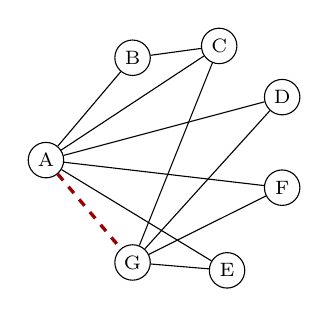
\begin{tikzpicture}[
          v/.style={circle,draw,inner sep=1pt,minimum size=4.5mm,font=\scriptsize},
          e/.style={thin}]
        \node[v] (A) at (0,0) {A};
        \node[v] (B) at (1.1,1.3) {B};
        \node[v] (C) at (2.2,1.45) {C};
        \node[v] (D) at (3,0.8) {D};
        \node[v] (F) at (3,-0.35) {F};
        \node[v] (G) at (1.1,-1.3) {G};
        \node[v] (E) at (2.3,-1.4) {E};
        \foreach \x in {B,C,D,E,F} \draw[e] (A) -- (\x);
        \foreach \x in {C,D,E,F} \draw[e] (G) -- (\x);
        \draw[e] (B) -- (C);
        \draw[very thick,dashed,red!60!black] (A) -- (G);
      \end{tikzpicture}

      \smallskip
      \scriptsize Example graph from \citet[Fig.~4]{liang2025centrality};
      dashed edge removed.
    \end{column}
    \begin{column}{0.66\textwidth}
      \centering
      \footnotesize
      \setlength{\tabcolsep}{4pt}
      \begin{tabular}{lrrrrrrr}
        \toprule
        Degrees & A & B & C & D & E & F & G \\
        \midrule
        Before & 6 & 2 & 3 & 2 & 2 & 2 & 5 \\
        After  & \alert{5} & 2 & 3 & 2 & 2 & 2 & \alert{4} \\
        \midrule
        Adj.\ eigenvalues & $\lambda_1$ & $\lambda_2$ & $\lambda_3$ & $\lambda_4$ & $\lambda_5$ & $\lambda_6$ & $\lambda_7$ \\
        \midrule
        Before & 3.60 & 0.85 & 0 & 0 & $-0.53$ & $-1.55$ & $-2.38$ \\
        After  & \alert{3.10} & \alert{0.94} & 0 & 0 & \alert{0} & \alert{$-1.20$} & \alert{$-2.84$} \\
        $|\Delta\lambda|$ & 0.50 & 0.09 & 0 & 0 & 0.53 & 0.34 & 0.46 \\
        \bottomrule
      \end{tabular}
    \end{column}
  \end{columns}

  \bigskip
  \begin{itemize}
    \item Five of the seven eigenvalues change, yet each moves by at most
          $\|\Delta A\|_2 = 1$ (Weyl): the eigen\emph{values} stay controlled.
    \item The multiplicity of $\lambda = 0$ jumps from 2 to \alert{3}: the solver may
          return any basis of the larger eigenspace, so the computed
          eigen\emph{vectors} need not resemble the previous ones.
  \end{itemize}
\end{frame}

\begin{frame}{Obstacle 5: Stability vs.\ expressivity}
  \begin{itemize}
    \item Sign-invariant methods
          \citep{dwivedi2020generalization,kreuzer2021rethinking,lim2023sign}
          do not guarantee ``same Laplacian, same encoding'' when eigenvalues
          have multiplicity.
    \item \textbf{BasisNet} is basis-invariant but \alert{unstable}: it applies
          different networks to different eigenspaces (hard partitioning).
    \item \textbf{PEG} \citep{wang2022equivariant} is provably stable, but
          processes all eigenspaces homogeneously, which \alert{loses expressive
          power} (e.g.\ weaker results on molecular regression,
          \citealp{rampasek2022recipe}).
  \end{itemize}

  \begin{block}{Open question}
    Can a positional encoding be stable \emph{and} expressive?
  \end{block}
\end{frame}

% ============================================================================
\section{Methods}

\begin{frame}{Overview of approaches}
  \centering
  \footnotesize
  \setlength{\tabcolsep}{5pt}
  \begin{tabular}{llccc}
    \toprule
    Method & Encoding & Sign inv. & Basis inv. & Stable \\
    \midrule
    LapPE \citep{dwivedi2020generalization} & Laplacian eigenvectors & aug. & -- & -- \\
    SAN \citep{kreuzer2021rethinking}       & Learned spectral attention & aug. & -- & -- \\
    SignNet \citep{lim2023sign}             & $\phi(v)+\phi(-v)$ & \checkmark & -- & -- \\
    BasisNet \citep{lim2023sign}            & Per-eigenspace networks & \checkmark & \checkmark & -- \\
    PEG \citep{wang2022equivariant}         & Eigenvector distances & \checkmark & \checkmark & \checkmark \\
    SPE \citep{huang2024stability}          & Soft eigenspace weighting & \checkmark & \checkmark & \checkmark \\
    \bottomrule
  \end{tabular}

  \medskip
  \footnotesize aug.\ = invariance only encouraged through random sign flipping. SAN: node LPE; its public code applies the flip only on MOLHIV and MOLPCBA.
\end{frame}

\begin{frame}{Toward a solution: Stable and Expressive PE}
  \begin{itemize}
    \item SPE \citep{huang2024stability} replaces hard eigenspace partitioning
          with a \alert{soft}, eigenvalue-dependent weighting:
          \begin{equation*}
            \mathrm{SPE}(V, \lambda) =
            \rho\big(\big[\, V \operatorname{diag}(\phi_1(\lambda)) V^\top,
            \dots, V \operatorname{diag}(\phi_m(\lambda)) V^\top \big]\big)
          \end{equation*}
    \item Each term is basis-invariant, since $V \operatorname{diag}(\cdot) V^\top$
          does not depend on the chosen basis.
    \item With Lipschitz $\phi_\ell$, close eigenvalues are treated similarly,
          giving \alert{provable stability} without discarding eigenspace
          information.
  \end{itemize}
\end{frame}

\begin{frame}{Beyond the Laplacian: NAPE}
  \small
  NAPE \citep{ajayi2024nape} \alert{never computes eigenvectors}, so it has no
  sign or basis ambiguity: it learns a node numbering for the sinusoidal PE of
  \citet{vaswani2017attention}.
  \begin{equation*}
    Z_i = \sigma(\gamma P_i + \epsilon) \in \{0,1\}^m
    \;\longrightarrow\; t = \mathrm{Dec}(Z_i)
    \;\longrightarrow\; \mathrm{Pos}(t)
  \end{equation*}
  \begin{columns}[T]
    \begin{column}{0.47\textwidth}
      \begin{itemize}
        \item Hamming distance on the hypercube mimics graph closeness:
              \begin{equation*}
                \mathcal{L} = \mathcal{L}_{adj}
                + \lambda_1 \mathcal{L}_{deg\_dist}
                + \lambda_2 \mathcal{L}_{deg}
              \end{equation*}
        \item Eigenvectors identify clusters, and so do BFS-like
              \alert{random walks}. With negative sampling, the cost is
              $O(|V|^2)$ if $l \cdot r \cdot k \leq |V|$.
      \end{itemize}
    \end{column}
    \begin{column}{0.49\textwidth}
      \centering
      \footnotesize
      \setlength{\tabcolsep}{3pt}
      \begin{tabular}{lrrrr}
        \toprule
        & \multicolumn{2}{c}{LapPE} & \multicolumn{2}{c}{scaled-NAPE} \\
        Dataset & Score & Time & Score & Time \\
        \midrule
        WikiCS       & 77.3 & 5.25 m & 77.7 & 2.50 m \\
        PubMed       & 85.3 & 22.0 m & 84.5 & 1.60 m \\
        OGBL-collab  & \multicolumn{2}{c}{out of memory} & 50.4 & 767 m \\
        \bottomrule
      \end{tabular}

      \smallskip
      \scriptsize Accuracy, or Hits@50 for OGBL-collab (baseline 53.9).\\
      $r$ walks of length $l$ per node, $k$ negative samples.
    \end{column}
  \end{columns}

  \medskip
  \textbf{Limits:} works on \alert{a single graph} at a time; encodings are not
  always unique (under 0.5\% of nodes shared one); needs a hyperparameter search;
  falls below the baseline on multi-graphs; does not address stability.
\end{frame}

% ============================================================================
\section{Conclusion}

\begin{frame}{Takeaways}
  \begin{itemize}
    \item Spectral encodings overcome the 1-WL limit by giving graph
          transformers a notion of position.
    \item Eigenvectors are not unique: \alert{sign} and \alert{basis}
          ambiguities must be handled by design, not by augmentation.
    \item Invariance alone is not enough: encodings must also be
          \alert{stable} under small perturbations of the graph.
    \item The central trade-off is \alert{stability vs.\ expressivity}; SPE is
          a step toward achieving both.
  \end{itemize}
\end{frame}

\begin{frame}[allowframebreaks]{References}
  \footnotesize
  \bibliographystyle{plainnat}
  \bibliography{references}
\end{frame}

\end{document}
